\section{Video Prediction for Control}
\label{sec:model}
In this section the video-prediction architecture is outlined building upon \cite{finn_nips}.
%%SL.10.15: This is a very abrupt way to start. Can you begin the section with a couple of sentences to explain what this section is about?

\begin{figure}[t]
    \centering
    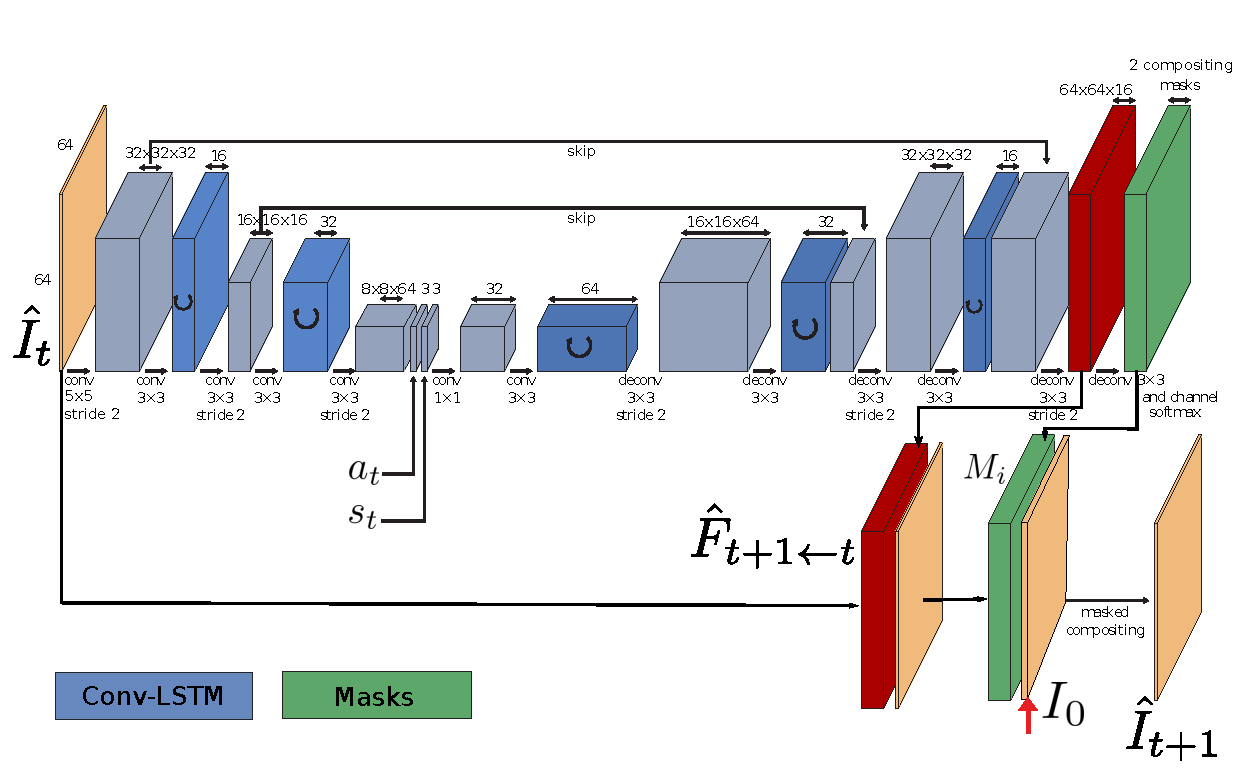
\includegraphics[width=\columnwidth]{images_sna/occlusionaware/architecture.pdf}
    \caption{\small{Simplified SNA model based on \autoref{eqn:simplemodel}. The red arrow indicates where the image from the first time step $I_0$ is concatenated with the transformed images $\hat{F}_{t+1 \leftarrow t} \diamond  \hat{I}_t $ multiplying each channel with a separate mask to produce the predicted frame for step $t+1$.}}      \label{fig:occlusion_model}
\end{figure}
%%SL.10.15: This figure is a bit cryptic, can we find a way to present a more detailed architecture diagram? Mohammad's paper has some good examples for how to make such diagrams more human-interpretable.

\subsection{Video Prediction via Pixel Transformations}
\label{subsec:pixel_trafo}
To predict the trajectory of these pixels we leverage the model proposed in \cite{finn_nips}. The model, shown in figure \ref{fig:occlusion_model}, uses stacked convolutional LSTMs that predict a 2 dimensional flow-field $\hat{F}_{t+1 \leftarrow t}$ at each time step and uses it to transform a current image $\hat{I}_t$ , similar to \cite{zhou2016view}.

%%SL.10.15: I would just present the whole model from the start.

%%SL.10.15: I think you need to actually describe the model. Maybe introduce the parts and the operators, and explain exactly the procedure for how a prediction about the next image emerges from the model. Instead of saying "the model predicts [something]" denote it with a function, with parameters

\begin{equation}
\hat{I}_{t+1} = \hat{F}_{t+1 \leftarrow t} \diamond  \hat{I}_t 
\label{simple_dna}
\end{equation}

where $\diamond$ denotes a bilinear interpolation operator that interpolates the pixel value bilinearly with respect to a location $(x,y)$ and its four neighbouring pixels in the image. The warping transformation $\hat{F}_{t+1 \leftarrow t}$ can be interpreted as a stochastic transition operator allowing us to make probabilistic predictions about future locations of individual pixels. 

\textbf{Predicting motion of individual pixels}: 
When using visual-MPC with a cost-function based on start- and goal pixel positions, a model is required that can effectively predict the 2-D motion of the selected start pixels $\pixel_0^{(1)}, \dots, \pixel_0^{(P)}$ up to $T$ steps into the future. Since the model we employ is transformation based, this flow prediction capability emerges implicitly, and therefore no external pixel motion supervision is required. To predict the future positions of the designated pixel $d$, the same transformations which are used to transform the images are applied to the distribution over designated pixel locations 

\begin{equation}
\hat{P}_{t+1} = \hat{F}_{t+1 \leftarrow t} \diamond  \hat{P}_t
\label{eqn:prob_forward}
\end{equation}

For simplicity we assume that we only use a single designated pixel. The distribution $\hat{P}_{t+1}$ is normalized at each time-step. Since this basic model, which we refer to as dynamic neural advection (DNA) model, predicts images only based on the previous image, it is unable to recover shapes (e.g., objects) after they have been occluded, for example by the robot arm. Therefore, this model is only suitable for planning motions where the user-selected pixels are not occluded during the manipulation, which restricts its use in cluttered environments or with multiple selected pixels. In the next section, we introduce an enhanced type of model, which lifts this limitation by employing temporal skip connections.

Depending on which type of planning cost function is used, the video prediction model needs to have certain properties. When using a classifier-based cost function, as detailed in section \ref{subsec:class_cost}, virtually any sensory prediction model can be used. When a cost function based on start- and goal pixel positions, it is necessary that the model is capable of predicting \emph{where} certain points in the image are moving.



\subsection{Skip Connection Neural Advection Model}
\label{subsec:skip}
To enable effective tracking of objects through occlusions, we can extend the model discussed in the previous section with temporal skip connections: we now transform pixels not only from the previously generated image $\hat{I}_t$, but from all but from all previous images $\hat{I}_0,...\hat{I}_{t}$, including the context image $I_0$, which is a real image, such that
\begin{equation}
\hat{I}_{t+1} =  \mathbf{M}_{0} (\hat{F}_{t+1 \leftarrow 0} \diamond I_t) +  \sum_{j=1}^{\tau} \mathbf{M}_{j} (\hat{F}_{t+1 \leftarrow j} \diamond  \hat{I}_j).
\end{equation}
We refer to this model as the \emph{skip connection neural advection model (SNA)}, since it handles occlusions by using temporal skip-connections such that when a pixel is occluded (e.g., by the robot arm or by another object) it can still reappear later in the sequence.
 
 \begin{wrapfigure}{r}{.37\columnwidth}
 	\centering
 	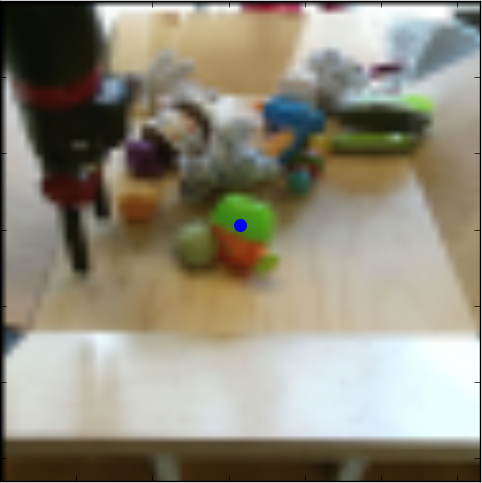
\includegraphics[width=0.4\columnwidth]{images_sna/occlusionaware/img_desigpixb0.png}
 	\caption{The blue dot indicates the designated pixel}
 	\label{fig:desig_pix_bluedot}
 \end{wrapfigure}

Transforming from all previous images comes with increased computational cost, since the number of masks and transformations scales with the number of time-steps $\tau$. However, we found that in practice a greatly simplified version of this model, where transformations are applied only to the previous image and the \emph{first image} of the sequence $I_0$ works equally well. Moreover we found that transforming the first image of the sequence is not necessary, as the model uses its pixels primarily to generate the image background. Therefore, we can use the first image directly, without transformation, such that
\begin{equation}
\hat{I}_{t+1} = \mathbf{M}_{0} I_t +  \mathbf{M}_{1} \hat{F}_{t+1 \leftarrow t} \hat{I}_t.
\label{eqn:simplemodel}
\end{equation}
Here, we make the assumption that occluded objects are static throughout the prediction horizon. This assumption allows us to dispense the intermediate transformations and only provide a skip connection from the very first image in the sequence $I_0$, which is also the only real image, since all of the subsequent images are predicted by the model. Hence, this model only needs to output 2 masks. 

We provide an example of the model recovering from occlusion in \autoref{fig:pix_reappear}. In this figure, the arm is predicted to move in front of the designated pixel, marked in blue in \autoref{fig:desig_pix_bluedot}. The predictions of the DNA model, shown in figure \autoref{fig:pix_reappear}(b), contain incorrect motion of the marked object, as shown in the heatmaps visualizing $\hat{P}_t$, although the arm actually passes in front of it. This is because the DNA model cannot recover information about an object that it has `overwritten' during its predictions, causing the model to predict that the pixel \emph{moves with the arm}. We identified this as one of the major causes of planning failure using the DNA model. By contrast our SNA model predicts that the occluded object will not move, shown in figure  \autoref{fig:pix_reappear}(a).

\todo{can cut from here:}
Next, we show another illustration comparing the occlusion handling of DNA and the proposed SNA model. The graphs in \autoref{fig:pix_reqppear_graph} show the predicted probability evaluated at the position of the designated pixel, shown in figure \ref{fig:desig_pix_bluedot}, which is stationary during the entire motion. Precisely when the arm occludes the designated pixel, the probability at this point decreases. This indicates that the model is `unsure' where this pixel is. When the arm unoccludes the designated pixel, it should become visible again, and the probability of the designated pixel being at its original position should go up. In the case of the DNA model and its variants~\cite{finn_nips}, the probability mass does not increase after the object reappears. 
 
 \begin{figure}[t]
 	\centering
 	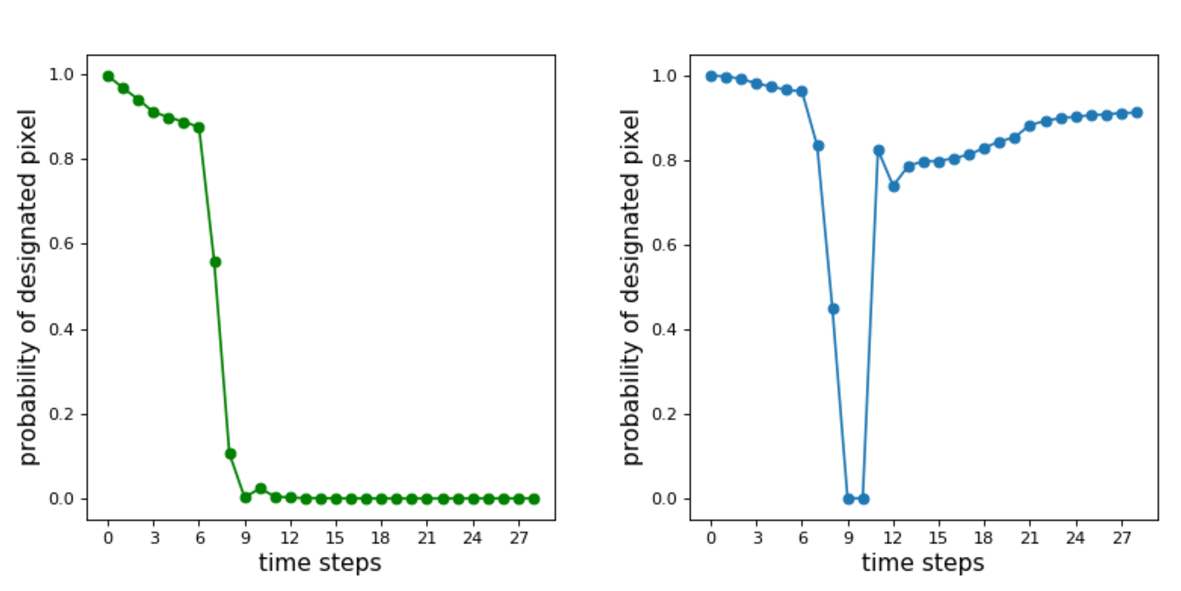
\includegraphics[width=0.9\columnwidth]{images_sna/occlusionaware/probability_curves.pdf}
 	\caption{Predicted probability $P_{d^{(0)}}(t)$ of the designated pixel being at the location of the blue dot indicated in \autoref{fig:desig_pix_bluedot} for the DNA model (left) and the SNA model (right). \todo{can cut if no more space!}}      \label{fig:pix_reqppear_graph}
 \end{figure}

\begin{figure}
    \centering
    \begin{subfigure}{0.9\columnwidth}
    \centering
        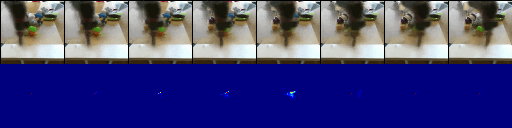
\includegraphics[width=1.\linewidth]{images_sna/occlusionaware/cdna_1ststep_bckgd_gen_pixb0_overtime.png}
        \caption{Skip connection neural advection (SNA) does not erase or move objects in the background}
        \label{fig:Ng1}
    \end{subfigure}
    \begin{subfigure}{0.9\columnwidth}
    \centering
        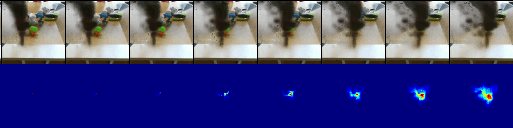
\includegraphics[width=1.0\linewidth]{images_sna/occlusionaware/orig_dna_gen_pixb0_overtime.png}
        \caption{Standard DNA \cite{foresight} exhibits undesirable movement of the distribution $P_{d}(t)$ and erases the background}
    \end{subfigure}
    \caption{
    %\protect\subref{fig:Ng1} 
    Top rows: Predicted images of arm moving \textit{in front of} green object with designated pixel (as indicated in \autoref{fig:desig_pix_bluedot}). 
    %(\protect\subref{fig:Ng2}) 
    Bottom rows: Predicted probability distributions $P_{d}(t)$ of designated pixel obtained by repeatedly applying transformations.}
    \label{fig:pix_reappear}
\end{figure}
